\documentclass{article}

\usepackage{booktabs,caption,csvsimple,graphicx,natbib}
\bibliographystyle{apalike}

\title{Volatility-Managed Stocks}
\author{Junyong Kim\footnote{University of Wisconsin--Milwaukee. junyong@uwm.edu.}}
\date{October 13, 2020\footnote{First draft: October 13, 2020.}}

\begin{document}

\maketitle

\begin{abstract}

I examine whether managing volatility improves stock returns as well as portfolio returns.

\smallskip

\textit{JEL codes:} G12. G14.

\textit{Keywords:} Volatility timing.

\end{abstract}

\bibliography{vm_sto}

\clearpage

\begin{figure}
\centering
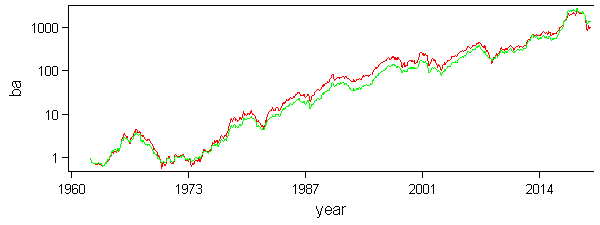
\includegraphics[width=0.5\textwidth]{_ba}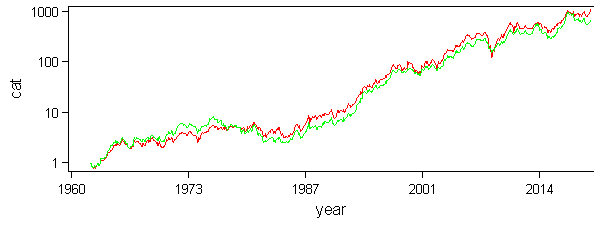
\includegraphics[width=0.5\textwidth]{_cat}
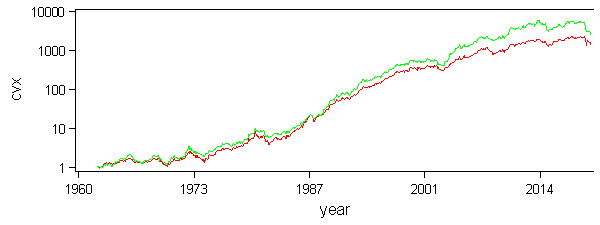
\includegraphics[width=0.5\textwidth]{_cvx}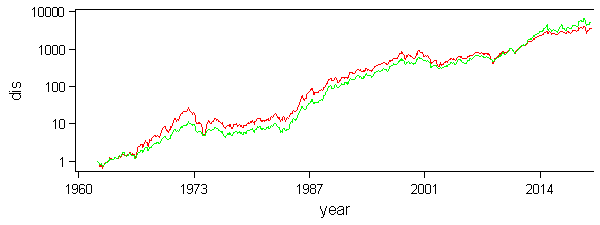
\includegraphics[width=0.5\textwidth]{_dis}
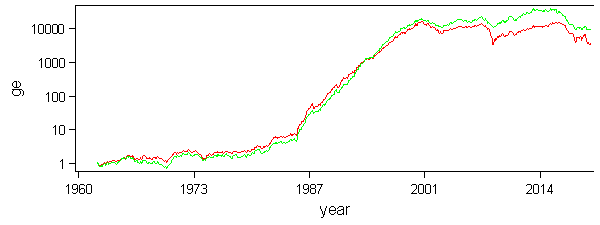
\includegraphics[width=0.5\textwidth]{_ge}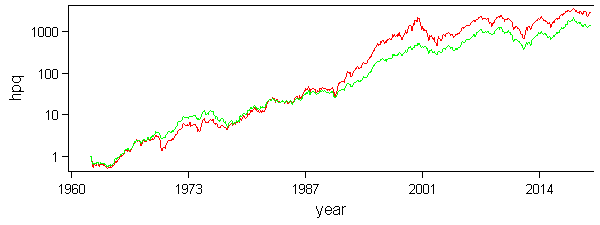
\includegraphics[width=0.5\textwidth]{_hpq}
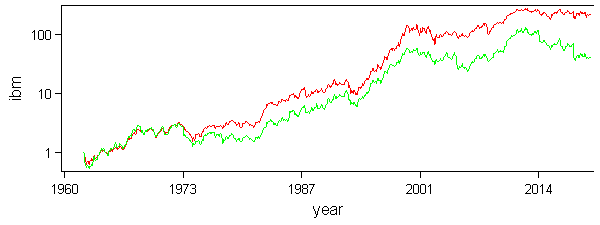
\includegraphics[width=0.5\textwidth]{_ibm}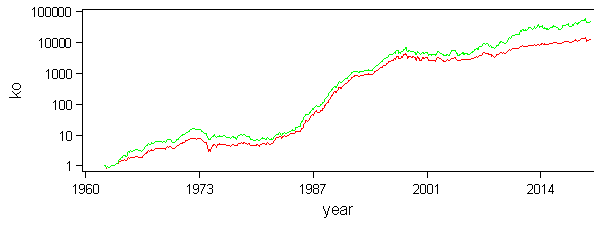
\includegraphics[width=0.5\textwidth]{_ko}
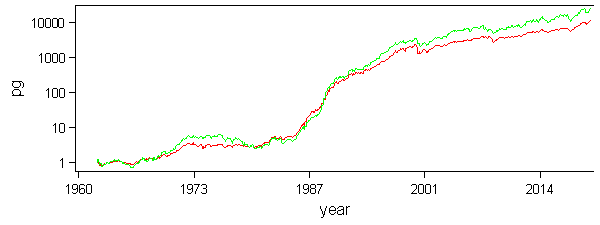
\includegraphics[width=0.5\textwidth]{_pg}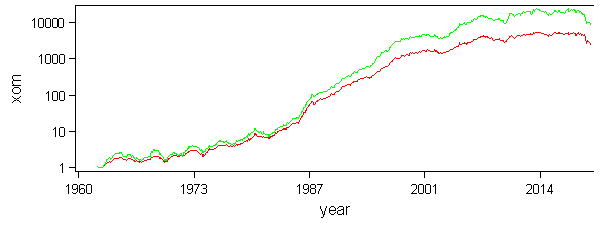
\includegraphics[width=0.5\textwidth]{_xom}
\caption{Cumulative returns to the volatility-managed stock returns}
\caption*{I mimic Figure 3 of \citet{moreira2017volatility} using stocks instead of portfolios.}
\end{figure}

\clearpage

\begin{table}
\centering
\caption{Volatility-managed stock alphas}
\caption*{I mimic Table I of \citet{moreira2017volatility} using stocks instead of portfolios.}
\csvautobooktabular{_alpha.csv}
\end{table}

\end{document}
